\section{Norine}
\label{nor_3}

\subsection{Généralités}

Nous avons déjà plusieurs fois abordé la base de données Norine au sein de ce manuscrit mais nous allons ici décrire en détail son fonctionnement.
Norine a été créée durant la thèse de Ségolène Caboche (2006-2009) dans le but de centraliser l'information sur les NRP.
C'est la première base de ce genre a avoir été mise en place et c'est aujourd'hui la base de référence.
Les structures atomiques et parfois monomériques de NRP étaient publiées dans des articles scientifiques puis quelquefois mises en ligne au sein de bases généralistes.
Il n'existait souvent aucune annotation monomérique renseignée en dehors de ces publications.
Norine a été créée dans le but de centraliser et rendre accessible les annotations NRP connues.
Sans cette centralisation, il est très difficile de créer des modèles de prédiction autour des NRP.
Les données de Norine ont par exemple été très utiles pour la création de modèles de prédiction d'activités NRP~\cite{abdo_prediction_2014,abdo_new_2012}.

\begin{figure}[h!]
  \begin{center}
    \includegraphics[width=350px]{Figures/Norine/sql.png}
    \caption{\label{sql}Schéma simplifié de la base de données Norine.
    Figure extraite de la thèse de Ségolène Caboche avec son accord.}
  \end{center}
\end{figure}

Norine est une base de données postgres contenant plusieurs dizaines de tables, toutes articulées autour de la notion de peptide (voir la version très simplifiée en figure \ref{sql}).
La table centrale des peptides contient toutes les informations propres au peptide telles que le nom, la famille ou les structures atomiques et monomériques.
Les informations d'activités, d'organismes producteurs ou le détail de chaque monomère sont quant à eux présents dans des tables annexes du fait qu'elles puissent être partagées entre différents peptides.
Par exemple, une table est dédiée aux activités.
Ces activités sont ensuite mises en relation avec les peptides via une table ``présente''.
Au sein de cette table d'association, il est possible de trouver plusieurs activités par peptide et plusieurs peptides par activité.

La base de données est accompagnée d'une interface web et d'un serveur Java J2EE.
L'interface a pour but de rendre les données simples d'accès pour tous les utilisateurs.
Elle est accessible via le serveur de logiciels de l'équipe Bonsai à l'adresse http://bioinfo.lifl.fr/norine/.
Chaque peptide et chaque monomère y possède sa page dédiée.
Sur ces pages se trouvent tous les détails présents en base de données.
Elles sont accessibles via des formulaires de recherche par nom/type/organismes producteurs/activité etc.
Pour les peptides, il existe également une recherche par sous graphe pour laquelle nous donnerons plus de détails par la suite.



\subsection{Les peptides}

\subsubsection{L'interface web}

\begin{figure}[h!]
  \begin{center}
    \includegraphics[width=450px]{Figures/Norine/malformin_nor.png}
    \caption{\label{interface}Page de présentation de peptide dans l'interface Norine.
    L'image a été contractée pour passer en une page.}
  \end{center}
\end{figure}

Comme nous l'avons déjà évoqué, toute la base de données est axée autour de notre matière première : les peptides.
Les pages centrales du site web sont donc logiquement les pages d'information correspondant à chaque NRP (voir figure \ref{interface}).
Ces pages sont divisées en trois parties.
En haut de la page se trouvent les informations générales comme le nom, l'identifiant ou la liste des activités connues de ce peptide.
La masse moléculaire est également présente et est particulièrement utile en spectrométrie de masse.
Cette première partie est purement factuelle et ne fait que reprendre les éléments basiques potentiellement présents dans d'autres bases.

La seconde partie de la page représente la plus grande contribution de Norine.
Cette partie donne toutes les informations à propos des structures.
Au minimum, elle contient la structure monomérique du NRP.
Dans le meilleur des cas, la structure monomérique est accompagnée d'un SMILES et depuis peu, d'un dessin de la structure atomique dont chaque monomère a été coloré par s2m.
La structure monomérique apparaît sous forme de graphe dans une interface visuelle ainsi que sous un format textuel.
Chaque monomère entrant dans la composition est affiché dans une liste.
Les liens au sein de cette liste permettent d'accéder au détail de chacun de ces monomères (nom, SMILES, composition, ...).

Enfin, la dernière partie de la page est consacrée aux références et liens.
Ce sont toutes les informations qui permettront de replacer le peptide dans son contexte et d'en savoir plus au travers d'autres bases de données.
Les organismes producteurs sont détaillés à cet endroit et un lien vers leur classification NCBI est disponible.
C'est également ici que sont répertoriés les articles de recherche qui ont permis la découverte du peptide et l'établissement de son statut non ribosomique.
Enfin, lorsqu'ils sont référencés, sont présents des liens vers d'autres bases de données.
Actuellement, pour apprendre plus de détails sur les structures chimiques des molécules, sont présents des liens vers pubchem et uniprot.


\subsubsection{Les méthodes de recherche}

Comme dans toutes les autres bases de données, il est possible de rechercher un peptide via de nombreux critères.
En indiquant le nom ou l'identifiant, un peptide unique pourra être trouvé.
En indiquant un nom partiel ou tout autre critère (avec la possibilité de combiner les critères), une liste de peptides sera retournée.
Cependant, Norine propose également un autre type de recherche très intéressant pour notre type de données.
Il est possible de rechercher les peptides par structures monomériques \cite{caboche_structural_2009}.
Plus précisément, il est possible de créer des expressions régulières de structures pour les rechercher dans la base.
Prenons un exemple.
Si nous souhaitons effectuer des recherches de peptides qui contiennent une Valine liée à n'importe quel variant d'une Cystéine ou d'une Leucine, il nous faut écrire la requête : Val,[Cys*|Leu*]@1@0.
Ce format est un format de graphe.
Les noms séparés par des virgules représentent les étiquettes des n\oe{}uds (un n\oe{}ud Val et un n\oe{}ud Cys* ou Leu*) et les valeurs séparées par des @, les arêtes.
Pour résumer cette requête, nous avons :
\begin{itemize}
 \item Le n\oe{}ud 0 étiqueté par Val
 \item Le n\oe{}ud 1 étiqueté par Cys* (n'importe quel dérivé de Cys) ou Leu*
 \item Un lien sortant du premier n\oe{}ud (n\oe{}ud 0) pour joindre le n\oe{}ud 1 (@1 en première position)
 \item Le même lien sortant du deuxième n\oe{}ud (n\oe{}ud 1) pour joindre le n\oe{}ud 0 (@0)
\end{itemize}

\begin{figure}[h!]
  \begin{center}
    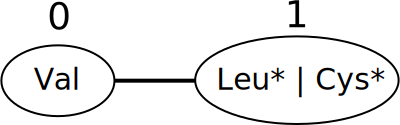
\includegraphics[width=200px]{Figures/Norine/requete.png}
    \caption{\label{requete}Requête Val,[Cys*|Leu*]@1@0.}
  \end{center}
\end{figure}

Une fois la requête formatée, il est possible d'exécuter deux algorithmes différents.
L'un des deux est un isomorphisme de sous-graphe.
Nous avons déjà longuement abordé le problème d'isomorphisme durant le second chapitre (voir \ref{SI_p}).
La requête est croisée avec toutes les structures monomériques présentes en base et retourne tous les peptides dont la structure monomérique contient le motif recherché.

Le second algorithme ne prend pas en compte la structure mais uniquement la composition.
C'est une recherche par \textit{fingerprint} composée des comptages de monomères et des comptages par groupes de monomères~\cite{abdo_new_2012}.
Plusieurs groupements sont définis dans Norine.
Par exemple Cys* cité précédemment est un groupement contenant la Cystéine, la D-Cystéine, l'alpha-méthyl-Cystéine et bien d'autres dérivés de la Cystéine.
Les fingerprints des peptides en base sont pré-calculés et le fingerprint de la requête est créé à la volée.
Le requête fingerprint est comparée à tous les fingerprints de la base et une distance est calculée.
Les résultats sont affichés par distance décroissante.
Cette recherche ne prend pas en compte les structures mais permet une souplesse dans les monomères inclus.
Les regroupements permettent de préserver une proximité élevée malgré la différence de monomère présent.



\subsection{Les outils liés}

Depuis la création de la base et du serveur web, beaucoup d'améliorations ont été effectuées~\cite{flissi_norine_2016}.
Ici nous allons parler des trois dernières évolutions majeures.


\subsubsection{Éditeur graphique}

\begin{figure}[h!]
  \begin{center}
    \includegraphics[width=450px]{Figures/Norine/editor.png}
    \caption{\label{editor}Éditeur graphique pour la construction de requêtes dans Norine.
    Ici, nous avons construit graphiquement la requête Val,[Cys*|Leu*]@1@0.}
  \end{center}
\end{figure}

Mise à jour en 2015 par Juraj Michalik\footnote{Juraj Michalik était ingénieur d'étude pour la plateforme bilille au moment de la création de l'éditeur graphique.}, l'interface de recherche dans la base possède désormais une interface graphique de création dynamique des requêtes.
L'interface permet de générer facilement des requêtes complexes (voir figure \ref{editor}).
Le menu de gauche permet de sélectionner les différents monomères que nous souhaitons ajouter à une requête et la page principale permet d'ajouter des liens entre monomères par de simples clics.
Au fur et à mesure de la création, la requête textuelle s'affiche au dessus de l'éditeur.
Une version sans interface d'interaction de cet éditeur est également utilisée sur les pages des peptides de Norine afin d'avoir une représentation graphique de ceux-ci.

Cet éditeur est d'un réel intérêt pour la base car il permet une interaction utilisateur simple qui n'était pas possible auparavant.
Une interface intuitive et conviviale est nécessaire pour rendre les outils bioinformatiques accessible au plus grand nombre et correspond à une demande des biologistes utilisateurs.



\subsubsection{Services REST}

Initié en 2014 par Areski Flissi\footnote{Areski Flissi est ingénieur de recherche au CNRS. Il est pour le moment affecté à l'équipe Bonsai, équipe de où j'effectue ma thèse, et s'occupe en grande partie de la maintenance et du développement de Norine et des outils satellites.}, une interface de récupération de données de la base Norine est disponible (interface REST).
Cette interface a pour but la simplification de l'interfaçage des données Norine avec d'autres logiciels.
Elle permet de récupérer un grand nombre de données de Norine par des requêtes HTTP complexes, sans avoir besoin de passer par l'interface web.
Nous avons utilisé cette interface pour récupérer les données de Norine afin de tester Smiles2Monomers.
Une explication d'utilisation de l'interface est disponible à l'adresse http://bioinfo.lifl.fr/norine/service.jsp



\subsubsection{Crowdsourcing via MyNorine}

Le dernier outil que nous allons présenter s'appelle MyNorine.
C'est un outil de crowdsourcing d'annotations NRP~\cite{flissi_norine_2016}.
Ceci veut dire que toute personne, même extérieure à l'équipe de développement de Norine, peut facilement soumettre de nouvelles entrées.
Tout comme l'interface REST, il a été développé par Areski Flissi.

MyNorine est en ligne depuis 2015 mais le développement de nouvelles fonctionnalités est toujours en cours.
L'outil utilise une interface intuitive pour l'utilisateur.
Il est possible d'entrer de nombreuses information mais seules les informations importantes sont obligatoires.
Parmi les informations obligatoires, on retrouve toutes les informations minimales comme le nom, le type de structure, la structure monomérique et au moins une référence bibliographique.
Pour ne pas avoir à construire la chaîne de caractères compliquée représentant la structure, l'interface javascript décrite ci-dessus est disponible aux moments opportuns.
Tout peptide soumis par un utilisateur sera ensuite envoyé à l'équipe de curateurs qui devra vérifier la validité et la pertinence de la soumission.
Pour l'instant, cette équipe de curateurs est composée de Maude Pupin, Valérie Leclère, Areski Flissi et moi même.

La mise à disposition de cette interface est une véritable plus-value pour la base de données.
Elle permet de donner du poids à la communauté en lui confiant une part du travail d'archivage des NRP.
À l'été 2015, nous avons organisé un workshop autour de la thématique NRPS/PKS durant lequel nous avons incité les membres de la communauté à partager leur travail au travers de MyNorine.
Quelques peptides ont été soumis, mais il est encore nécessaire de communiquer pour rendre récurrent ce partage d'informations pour chaque nouveau peptide découvert.









\section{Les contributions de s2m à Norine}
\label{cont_nor}

Jusqu'à présent, nous avons présenté les méthodes informatiques qui permettent de traiter, analyser et générer les données contenues dans Norine.
Cette section sera consacrée à la bioanalyse qui est nécessaire pour assurer la validation manuelle  des données et donc leur qualité.
Comme tout au long de ma thèse, ce travail a été réalisé en étroite collaboration avec les membres du sous-groupe Norine.
Les travaux que je vais présenter ici sont issus des analyses réalisées lors de nos réunions surnommées les ``Norine days'' et de collaborations avec des stagiaires et ingénieurs.

Les Norine days sont des réunions de travail qui réunissent tous les acteurs de Norine.
Ces réunions se font lors de demi-journées et nous permettent d'aborder des problèmes et de proposer des solutions collectives.
Elles m'ont été d'une grande aide pour acquérir les notions de biologie et de chimie nécessaires à mon travail.
Lors de ces réunions, j'ai apporté les résultats de s2m, ce qui nous a mené à la découverte d'erreurs d'annotation présentes en base.
Je présenterai par la suite les différentes étapes de la correction et de la mise en place de gardes-fous pour aider à faire disparaître les erreurs d'annotation dans les structures.

Durant ces journées nous prenons également beaucoup de temps pour analyser les nouvelles entrées soumises par des contributeurs extérieurs.
Ces contributions nous ont d'ailleurs plusieurs fois menées à réaliser des changements au sein de l'ontologie de Norine et à la normalisation de concepts déjà présents.

La seconde partie de cette section sera consacrée aux collaborations avec des stagiaires et ingénieurs qui ont menées à la création de nouveaux contenus pour la base de données.
Dans les deux cas que nous verrons, nous aborderons l'utilisation de s2m pour l'ajout automatique d'annotations.


\subsection{Améliorations de l'existant}

Norine est constituée d'environ 1200 peptides annotés.
Toutes ces annotations ont été extraites une à une d'articles scientifiques puis entrées dans la base de manière manuelle.
Bien que le travail ait été réalisé avec beaucoup de rigueur, un certain nombre d'erreurs se sont glissées en base.
Comme présenté lors des résultats de s2m (voir \ref{resultats_s2m_p}), le logiciel permet la détection de certaines erreurs.
Voyons ici les procédures mises en place pour corriger ces erreurs et essayer d'empêcher l'introduction de nouvelles.


\subsubsection{s2m pour corriger les erreurs}

\begin{figure}[h!]
  \begin{center}
    \includegraphics[width=450px]{Figures/contributions/dap_modif.png}
    \caption{\label{dap_modif}Partie A : le processus de modification du monomère Dap au sein de Norine, via l'utilisation de MyNorine.
    Partie B : la conséquence de la modification du SMILES du Dap sur la couverture de l'annotation trouvée par s2m.}
  \end{center}
\end{figure}

Lors de l'analyse des résultats nous avons détecté quatre types d'erreurs : les erreurs de structure atomique peptidique, d'annotation peptidique, de structure atomique monomérique et d'équivalences structurelles.
Cette dernière erreur est entièrement due à la façon dont s2m est conçu et rien n'est à corriger en base.
Pour les 3 autres erreurs, myNorine nous permet facilement de modifier les entrées de la base.

Appliquons une correction d'un peptide pour lequel nous avons découvert une erreur d'annotation.
Pour la dolastatin 10, à la suite d'une recherche au sein des publications, nous avions déterminé que le monomère Dap de Norine était structurellement incorrect (voir \ref{dolastatin_p}).
Effectuons la modification de ce monomère via myNorine (voir figure \ref{dap_modif}).
Nous pouvons lancer la modification depuis la page Norine du monomère.
Changeons le SMILES du monomère en plaçant correctement l'azote puis validons.
Après validation de la modification, l'entrée est correcte en base.

Pour toutes les erreurs détectées par s2m, nous devons répéter ce processus de recherche des structures correctes puis de changement des entrées de Norine.
Souvent, une modification dans un peptide nous amène à découvrir plusieurs autres modifications mineures nécessaires.
Il nous est par exemple plusieurs fois arrivé de découvrir des incohérences de nomenclature et de finalement passer un long moment sur une procédure de normalisation.
C'est un processus qui prend énormément de temps et qui doit être effectué collectivement afin de ne pas prendre de décisions contradictoires.
Le traitement des erreurs est à ce jour toujours en cours et nous avançons au rythme de 1 à 5 peptides par réunion (environ 100 cas d'erreurs à traiter).


\subsubsection{s2m pour empêcher les erreurs}

Après avoir traité les erreurs existantes, nous allons discuter de la manière de limiter l'introduction de nouvelles erreurs.
Le seul moyen est d'essayer de détecter automatiquement les annotations fausses lorsqu'elles sont entrées et de proposer à l'utilisateur le choix entre notre correction et ce qu'il a entré.

\begin{figure}[h!]
  \begin{center}
    \includegraphics[width=450px]{Figures/contributions/warning.png}
    \caption{\label{warning}Alerte levée au sein de MyNorine lorsqu'une annotation d'utilisateur ne parait pas correspondre à l'annotation automatique de s2m.}
  \end{center}
\end{figure}

Dans le cas de Norine, toute nouvelle entrée manuelle est effectuée via MyNorine.
Pour éviter l'introduction d'erreurs, si le SMILES de la molécule est entré, nous exécutons s2m en arrière plan.
Si l'annotation obtenue par s2m couvre entièrement le peptide mais que cette annotation diffère de l'annotation entrée manuellement, nous avertissons l'utilisateur et lui demandons de vérifier sa structure avant validation (voir figure \ref{warning}).
Cela nous a permis plusieurs fois durant les Norine days de nous rendre compte d'erreurs que nous étions en train de commettre et nous pensons que cela permettra d'en éviter de nombreuses autres.

\subsubsection{s2m pour des saisies semi-automatiques}

\begin{figure}[h!]
  \begin{center}
    \includegraphics[width=450px]{Figures/contributions/s2m_automatic.png}
    \caption{\label{s2m_automatic}Création d'annotation à partir d'un SMILES lors d'une création de nouvelle entrée via MyNorine.}
  \end{center}
\end{figure}

Dans MyNorine, nous proposons à l'utilisateur d'exécuter s2m avant d'entrer son annotation de manière complètement manuelle.
Si un SMILES est renseigné, alors s2m peut être déclenché pour obtenir une première annotation (voir figure \ref{s2m_automatic}).
L'utilisateur peut ensuite la modifier si celle-ci n'est pas complètement exacte.
Par ce système nous incitons les contributeurs à ajouter le SMILES de leurs peptides (information pas toujours présente dans Norine pour le moment) et nous évitons les erreurs d'inattention et fautes de frappe lors de la saisie utilisateur.

Comme le montrent les deux dernières sections, s2m a permis à MyNorine d'augmenter encore la qualité des annotations entrées en évitant des erreurs humaines.




\subsection{Mises à jour de Norine}

Les Norine days, nous ont amené à travailler très régulièrement sur les données de Norine, ainsi que sur des données d'autres bases.
Cette exploration en profondeur nous a révélé plusieurs faits.
Premièrement, les données de Norine, comme celles de nombreuses bases, sont vieillissantes.
Par exemple en suivant des liens Pubchem, nous nous sommes aperçus qu'ils ne pointaient plus tous vers les bonnes structures.
Nous avons également mis à jour le fait que l'évolution de la taxonomie au cours des années, a rendu obsolète certaines classifications d'organismes dans Norine.
Plusieurs autres détails ont également changé et nous font dire qu'une mise à niveau s'impose.
Cette mise à niveau sera le premier point que nous aborderons dans cette section.

Deuxièmement, en parcourant des bases telles que MiBIG qui répertorient des NRP et NRPS, nous avons constaté qu'il existe une grande quantité de NRP facilement accessibles et candidats pour un ajout au sein de Norine.
Ces données sont en général bien structurées et pourraient facilement être indexées par Norine.

Enfin, il existe également de nombreuses molécules NRP présentes dans des bases de données généralistes.
Nombre d'entre elles sont sans annotation monomérique.
En utilisant s2m sur de très grandes bases telles que PubChem, nous essayerons d'obtenir des annotations monomériques afin d'extraire des candidats NRP.
Ces molécules pourront ensuite être analysées manuellement, pour être enfin entrées en base ou ignorées.


\subsubsection{Mise à jour des données de Norine}

Nous allons ici parler du vieillissement des données de Norine.
Il existe au sein de Norine des champs dont les informations sont obsolètes ou imprécises.
Nous pouvons regrouper ces informations sous quatre catégories : les liens externes rompus (liens vers PubChem et Uniprot), les taxonomies non mises à jour, les molécules/organismes ayant changé de nom et les mises à jour de peptides associés à de nouvelles publications.
Analysons un à un chacun de ces cas.


\textbf{Vérification des liens externes}~~~
Les liens rompus représentent la catégorie la plus facile à traiter.
Un script simple a suffi pour les corriger.
Un à un, nous suivons automatiquement les liens vers les bases.
Certains d'entre eux ne mènent plus à rien et nous pouvons alors les supprimer.
Dans ce cas, nous cherchons ensuite le nom du peptide via l'API de PubChem pour espérer trouver une autre page correspondante.
Lorsqu'une structure est retrouvée, nous la faisons annoter par s2m afin de vérifier la cohérence de structure avec l'annotation manuelle de Norine.
Si l'annotation correspond, le nouveau lien est ajouté.
De la même manière, il est possible de vérifier les liens encore fonctionnels ou d'ajouter des liens à certains peptides n'en possédant pas.
De cette manière nous avons remis à jour plusieurs dizaines de liens.


\textbf{Mise à jour de la taxonomie}~~~
La taxonomie pose plus de problèmes car elle évolue au cours du temps.
La taxonomie du vivant a évolué au fur et à mesure des découvertes et des nouvelles méthodes de classification.
Il n'y a aucun doute sur le fait qu'elle continuera à évoluer rapidement.
Au sein de Norine, ce n'est pas une ressource critique mais il est bon de connaître les lignées d'espèces productrices de NRP pour pouvoir faire des rapprochements entre NRP/NRPS.
Ces données de taxonomie peuvent être récupérées depuis le site ou l'API du NCBI.
Le NCBI étant un organisme de référence, beaucoup de contributeurs maintiennent les classifications à jour.
En effectuant régulièrement une recherche sur le NCBI de la taxonomie des espèces présentes dans Norine, il est possible de maintenir les données suffisamment à jour.

Les données de taxonomie de Norine sont, pour le moment, maintenues comme des chaînes de caractères au sein de la table des organismes.
Cette structure est très redondante et ne permet pas de mises à jour efficaces.
Nous avons profité de la création du script de mise à jour pour revoir complètement notre façon de stocker les taxons.
La chaîne de caractères du champ organisme est remplacée par un identifiant dans la nouvelle table des taxons de Norine.
Cette table est organisée comme un arbre pour permettre une mise à jour taxon par taxon sans avoir besoin de modifier des dizaines d'entrées.
La construction de toute la chaîne taxonomique d'une espèce prend désormais beaucoup plus de temps (beaucoup plus de requêtes) mais ce problème est facilement contournable par la création de vues SQL.
Par ce script, c'est l'ensemble des données de Norine qui ont été remises à jour.


\textbf{Détection des changements de nomenclature}~~~
Les deux scripts de mise à jour dont nous venons de décrire ne peuvent pas fonctionner dans 100\% des cas.
Depuis leur publication (parfois remontant aux années 1980), certaines molécules et certains organismes ont changé de nom.
Heureusement, à la fois le NCBI et PubChem gardent en mémoire une liste conséquente de synonymes permettant ainsi de les retrouver.
Cependant, nos scripts ne trouvent pas toujours de synonymes, ce qui nous empêche d'effectuer les mises à jour.
Dans ce cas, nous levons des alertes qui devront être analysées à la main (probablement durant des ``Norine days'').


\textbf{Ajout de publications}~~~
En analysant les annotations issues de s2m, nous nous sommes parfois aperçu de l'existence de nouveaux articles à propos des molécules étudiées.
Certains articles nous permettaient alors de mettre à jour l'annotation présente dans Norine, de créer des entrées pour des variants nouvellement connus et parfois d'infirmer la production non ribosomique du peptide (dans ce cas le peptide n'a plus sa place dans Norine).
Ce dernier cas est très problématique car, pour le moment, il n'a pas été prévu dans Norine de retirer les informations d'une quelconque manière.
Il est toujours possible de retirer les informations directement en SQL mais cette solution ne permet pas aux utilisateurs de comprendre la disparition de la molécule.
Après concertation sur la nomenclature et les procédures d'évolution des données nous nous sommes mis d'accord pour ajouter un statut ``deprecated'' au sein de la base.
Pour le moment il existe les statuts ``curated'' et ``putative'' associé à chaque peptide.
L'ajout de ce nouveau statut permettra de regrouper tous les peptides qui ont un jour été considérés NRP mais qui, depuis, ont été prouvés produits par d'autres voies de synthèse.
Encore une fois, cette mise à jour n'est pas automatisable et nécessite un traitement particulier.
La procédure devrait un jour être ajoutée à myNorine.


\subsubsection{Récupération massive de NRP}
\label{nor_fill}

L'exploration des bases de données proches des NRP permet de se rendre compte que de nombreuses molécules NRP connues ne sont pas répertoriées au sein de Norine.
Afin d'essayer de combler le retard d'annotation de ces peptides, nous avons décidé d'automatiser leur intégration dans Norine.
À partir d'un script, nous analysons et ajoutons les NRP présents au sein des bases MiBIG (voir \ref{bdd_nrp}) et BIRD.
BIRD~\cite{young_chemical_2013} (the Biologically Interesting molecule Reference Dictionary) est une base de données regroupant de petits polymères antibiotiques et inhibiteurs.
Les deux bases ont pour avantage de contenir des entrées permettant la différentiation des NRP du reste des molécules.
Cela nous facilite la tâche en nous assurant du statut des molécules que nous ajoutons à Norine.

Une fois les molécules récupérées, nous utilisons s2m pour produire l'annotation monomérique nécessaire à l'entrée d'un NRP en base.
Cependant, en ajoutant automatiquement de nombreuses et nouvelles molécules automatiquement, nous ne respectons plus la charte de qualité que s'étaient fixés les créateurs de Norine.
C'est pourquoi chacune des données importées automatiquement porte un statut nouveau appelé ``automated''.
Lorsqu'un utilisateur recherchera des peptides sur l'interface web, les annotation manuelles seront mises en avant par rapport à celles générées automatiquement.
Les pages de ces nouveaux peptides seront également marquées avec la provenance des données et un lien y apparaîtra.

Par ce script, 471 nouvelles annotations NRP vont être ajoutées à la prochaine version de Norine (+40\% de peptides).
Une troisième partie de script est en cours d'intégration afin d'indexer les données issues de ClustScan database.
Ce travail a été effectué en collaboration forte avec Juraj Michalik lorsqu'il était en contrat d'ingénieur au sein de notre équipe.



\subsubsection{Fouille en bases de données}
\label{nor_auto}

La dernière méthode de mise à jour de Norine est la plus exploratoire.
L'idée est de scanner d'immenses bases de données chimiques à la recherche de peptides dont la structure monomérique nous fait penser à un NRP.
Ces structures seront générées par s2m à partir des SMILES présents dans ces bases.
L'optimisation effectuée sur le temps de calcul de s2m permet de passer à l'échelle et de scanner des dizaines de milliers de molécules.
Sans aucune modification de s2m, nous sommes capables de charger et d'analyser environ 250 molécules par minute.
En désactivant la recherche \textit{light} pour tous les peptides qui n'ont pas une couverture suffisante, il est possible d'annoter 3 fois plus de structures dans le même temps.

Pour effectuer un premier test, nous avons choisi d'extraire de PubChem toutes les molécules qui répondent à la requête ``peptide''.
Ce premier filtre limite le nombre d'entrées que nous avons à évaluer lors d'un premier test.
Au total c'est 1~626~461 composés qui ont été récupérés.
Les annotations de ces peptides par s2m on été faites en un peu plus de 36 heures sur une seule machine standard (3.2 Ghz de CPU mono-thread et 8 Go de RAM dédiés au programme).

Une fois les annotations obtenues, nous cherchons à séparer les NRP du reste des molécules en utilisant plusieurs critères de filtration.
Obtenir un bon taux de couverture lors du passage de s2m sera notre premier critère.
Pour commencer, soyons très exigeants et réclamons de n'obtenir que les peptides 100\% couverts.
Nous obtenons 12830 peptides.

En regardant rapidement, on s'aperçoit que de nombreuses molécules sont constituées de seulement un ou deux monomères.
Ajoutons un filtre sur le nombre minimal de monomères par molécule.
Dans les statistiques de Norine, la plupart des peptides possèdent au moins 7 monomères.
Filtrons donc toutes les annotations de moins de 7 monomères.
Nous obtenons désormais 5342 peptides.

Enfin, les NRP sont noyés au milieu de nombreuses protéines classiques.
Rappelons que les protéines classiques sont constituées uniquement de 20 acides aminés différents.
Leur voie de synthèse n'effectue que des assemblages linéaires.
Excepté quelques modifications enzymatiques post-synthèse, les peptides classiques sont linéaires.
En filtrant tous les peptides qui ne contiennent que des acides aminés 
protéogéniques ainsi que ceux qui sont linéaires, nous devrions augmenter la densité de NRP dans notre sortie.
Nous ajoutons comme filtre l'impossibilité d'être linéaire (nombre de liaisons supérieur ou égal au nombre de nœuds) et l'obligation de posséder au moins deux monomères ne faisant pas partie des 20 de base.
Finalement nous obtenons 1097 peptides.

\begin{figure}[h!]
  \begin{center}
    \includegraphics[width=450px]{Figures/contributions/didemnin_B.png}
    \caption{\label{didemin}À gauche~: une des sorties après processus de filtration.
    À droite~: le NRP correspondant dans la base Norine.}
  \end{center}
\end{figure}

Bien évidemment, ces 1097 structures ne sont pas toutes des peptides non ribosomiques.
Les protéines classiques sont modifiées par de nombreuses enzymes qui permettent parfois la cyclisation et la transformation de monomères.
Ces protéines peuvent être modifiées au point de les faire ressembler à des NRP.
Nous ne pouvons donc pas être certains que les molécules issues du processus de filtration soient bien NRP.
Cependant un bon indice de la qualité de la méthode est que nous retrouvons à l'aveugle des NRP de Norine.
Nous avons par exemple retrouvé la ``didemnin B'' (figure \ref{didemin}).
En effectuant une recherche par structure depuis l'interface de Norine, nous avons retrouvé ce NRP.
Quelques exemples n'étant pas des preuves, il faudra revenir sur ces données afin de les valider manuellement.
C'est à nouveau un très long travail de bioanalyse qui viendra compléter les données de Norine.



\newpage
\section{Vers la biologie de synthèse}
\label{bio_synth}

Depuis quelques années, les bactéries développent de plus en plus de résistances aux antibiotiques utilisés en médecine animale.
Les NRP étant une source très riche d'antibiotiques, de nombreuses équipes essayent de créer, à partir de NRP, de nouvelles molécules contre lesquelles les micro-organismes ne présentent pas de résistance.
C'est dans le but de contribuer à la création de ces nouvelles molécules que nous allons ici aborder la thématique de la biologie de synthèse.
La biologie de synthèse est un domaine qui vise à modifier des organismes pour les pousser à effectuer des tâches que nous souhaitons.
Dans notre cas, le but est de faire produire en masse par une bactérie, des NRP qui nous intéressent.

Cette section va décrire la suite du travail présenté précédemment.
L'annotation NRP n'est pas une fin en soi mais une donnée précieuse pour comprendre l'assemblage moléculaire et de fait, les voies de synthèse.
Le Graal de la biologie de synthèse appliqué aux NRP est de savoir comment produire nos propres assemblages monomériques en manipulant des gènes NRPS.
Comme nous le verrons par la suite, cette question est très ambitieuse par rapport à l'avancée des connaissances actuelles.
Notre première étape sera de mettre en relation les NRP avec les clusters de gènes capables de produire des peptides similaires.
Cette information sera très utile pour aider au design de nouveaux NRP à partir de briques déjà existantes.


\subsection{L'existant}

Commençons par un tour d'horizon des travaux dans ce domaine.
Nous nous appuierons sur des travaux de revue généralistes~\cite{carbonell_bioinformatics_2016} et spécialisés pour les NRP~\cite{kries_biosynthetic_2016}.
Effectuons un survol des techniques en commençant par de petites modifications monomériques pour arriver finalement à la création totale d'un NRP.


\subsubsection{Les modifications peptidiques}
% Recent advances in engineering nonribosomal peptide assembly lines
% Ribosome-independent biosynthesis of biologically active peptides: Application of synthetic biology to generate structural diversity

L'une des approches pour obtenir de nouvelles structures peptidiques est de faire varier des structures déjà produites.
La structure peut être modifiée post-synthèse NRPS, par des enzymes présentes dans le cluster de gènes.
Cela se produit naturellement, par exemple, lors d'incorporations de sucres dans un NRP (voir section \ref{sucres}).
En ajoutant des gènes d'enzymes de modification NRP au cluster de gènes ou en modifiant l'activité d'enzymes déjà présentes, certaines équipes parviennent à l'ajout de nouveaux monomères ou la modification de certains monomères déjà inclus~\cite{giessen_ribosome-independent_2012} (voir figure \ref{post_synth}).

\begin{figure}[h!]
  \begin{center}
    \includegraphics[width=300px]{Figures/synthese/post_synth.png}
    \caption{\label{post_synth}Modification post-synthèse du NRP par une action enzymatique.
    Les gènes NRPS contenant l'encodage des domaines A ``vert'' et ``rouge'' sont transcrits puis traduits depuis l'ADN afin de former les NRPS contenant les domaines de même couleur.
    La NRPS assemble ensuite le peptide.
    C'est enfin une enzyme ajoutée au cluster de gènes (ici en bleu), qui vient modifier l'un des monomères du NRP.}
  \end{center}
\end{figure}

L'article \cite{winn_recent_2016} propose également d'aller plus loin en effectuant parfois cette modification avant l'assemblage NRPS.
Les auteurs publient par exemple plusieurs modifications pré-synthèse de la Pacidamycin.
Ce sont des enzymes modificatrices qui agissent sur un monomère cible avant sa capture (par exemple, dans l'article, Trp est dérivé en Cl-Trp ou d'autres variants).
La structure du monomère n'étant pas fondamentalement changée, il est inclus par la synthétase sans changement préalable de celle-ci.
Les contraintes structurelles des NRP n'autorisent pas toujours une modification post-synthèse de ce monomère.
La modification pré-synthèse de monomères, lorsqu'elle n'affecte pas la capture du dit monomère, ouvre beaucoup de possibilités de modification.
% La surface en contact lors de la capture et de l'assemblage n'étant pas modifiée, les monomères alternatifs sont intégrés de la même manière que l'original.
% Certains monomères ne sont plus facilement modifiables par des enzymes post-synthèse du fait des contraintes structurelles.
% La modification de monomères pré-synthèse ouvre la voie vers de nouvelles structures peptidiques.


\subsubsection{Les modifications ponctuelles de synthétases}
% Introduction of a Non-Natural Amino Acid into a Nonribosomal Peptide Antibiotic by Modification of Adenylation Domain Specificity
% Mapping the Limits of Substrate Specificity of the Adenylation Domain of TycA
% Reprogramming Nonribosomal Peptide Synthetases for “Clickable” Amino Acids

\begin{figure}[h!]
  \begin{center}
    \includegraphics[width=250px]{Figures/synthese/mutations.png}
    \caption{\label{mutation}Des mutations ont été introduites au sein de l'ADN codant la NRPS, au niveau du domaine A vert.
    Le domaine A produit ne correspond plus à un domaine A vert mais à un variant proche.
    Le monomère capturé par ce domaine ne correspond plus à un monomère vert mais directement au variant proche correspondant au domaine modifié.}
  \end{center}
\end{figure}

La seconde possibilité de modification de NRP passe par la modification des synthétases.
Plus exactement par la modification de la séquence génétique correspondant à un domaine A d'une synthétase.
Les travaux \cite{villiers_mapping_2009, kries_reprogramming_2014, williams_engineering_2013} partent du constat (également fait par Stachelhaus~\cite{stachelhaus_specificity-conferring_1999}) que les domaines A sont spécifiques aux monomères qu'ils capturent.
En modifiant certains acides aminés composant un domaine A, la spécificité de ce domaine peut changer (voir figure \ref{mutation}).
Après quelques mutations bien effectuées, la poche d'accueil du monomère est suffisamment modifiée pour accueillir un autre monomère.
Les modifications à effectuer sont découvertes via des techniques d'évolution dirigée.
Les auteurs génèrent des mutations aléatoires (partiellement dirigées) sur les modules A puis ne gardent que ceux qui changent de fonction.
Par ce procédé, ils arrivent à capturer des monomères nouveaux, parfois non naturels~\cite{thirlway_introduction_2012}.



\subsubsection{Les modifications de domaines de synthétases}
% Reinvigorating natural product combinatorial biosynthesis with synthetic biology
% Harnessing the Biosynthetic Code: Combinations, Permutations, and Mutations

\begin{figure}[h!]
  \begin{center}
    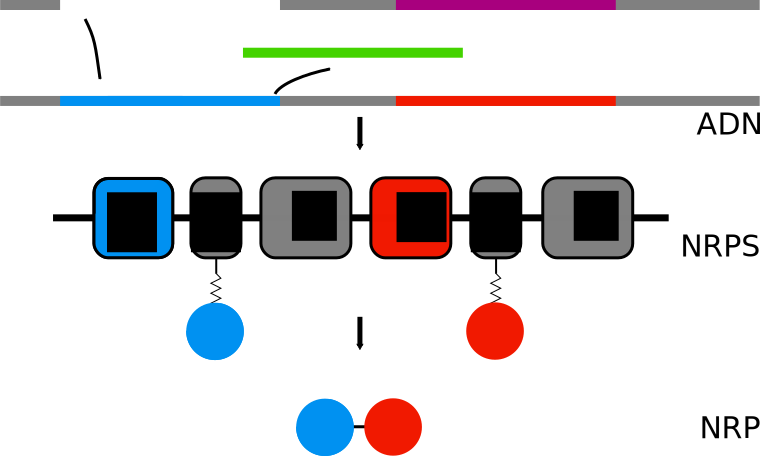
\includegraphics[width=250px]{Figures/synthese/echange.png}
    \caption{\label{echange}La séquence correspondant au domaine A incluant un monomère vert est remplacée par la séquence d'un domaine A correspondant à un monomère bleu.
    En conséquence, le monomère inclus par la synthétase est bleu.}
  \end{center}
\end{figure}

Les modifications qui paraissent les plus évidentes sont celles qui font appel à des échanges de domaines (voir figure \ref{echange}).
Des exemples sont présentés au sein des articles \cite{cane_harnessing_1998,kim_reinvigorating_2015}.
Intuitivement, nous pourrions nous dire qu'il est facile d'échanger par exemple deux modules A de deux synthétases comme on échangerait deux pièces de LEGO\textregistered ~dans une construction.
Malheureusement, ces modifications ne sont pas si directes car les modules échangés doivent respecter la structure 3D de la NRPS.
%des contraintes spatiales et physico-chimiques pour que la NRPS ait une cohérence structurelle.
Les structures 3D n'étant pas souvent connues, il est très difficile de prédire un comportement de NRPS avant d'effectuer l'échange expérimentalement.
%De plus, certaines recombinaisons ne fonctionnent pas, mais la ou les raison(s) de cet échec sont inconnues à ce jour.

% A Subdomain Swap Strategy for Reengineering Nonribosomal Peptides

Bien que les contraintes structurelles soient des contraintes fortes, certaines équipes ont réussi des preuves de concept de cette technique.
Par exemple, les auteurs de l'article~\cite{kries_subdomain_2015} procèdent à l'échange d'une sous partie de domaine A afin de modifier son site actif.
Ils ont ainsi réussi à modifier le domaine A du premier module de la Gramicidine S et ainsi obtenir une production peptidique chimérique.
Ce résultat est très encourageant pour la suite et devrait pouvoir mener à la production de variants de peptides existants.
% Pour outrepasser ce genre de difficultés, les auteurs de \cite{kries_subdomain_2015} procèdent uniquement à un échange de sous domaine A.
% Ils modifient une partie de la zone spécifique en essayant de préserver la structure globale du module.
% Par cette technique, ils arrivent à modifier la forme de la poche et capter de nouveaux monomères.


\subsubsection{La création \textit{de novo} de peptides}

Nous arrivons désormais au Graal de l’ingénierie NRP : créer un peptide de toutes pièces.
Pour le moment, il n'existe aucune technique pour effectuer cette tâche.
Comme nous l'avons vu précédemment, modifier un domaine A est déjà très difficile et nécessite de l'expertise accompagnée d'un peu de chance.
Cependant, certains travaux cherchent déjà à concevoir des briques de base qui nous permettraient un jour de construire un peptide complet.
Ainsi, les travaux menés par Wilcoxen \textit{et al}~\cite{wilcoxen_biomimetic_2007} ont permis la création d'un peptide synthétique mimant le comportement d'un domaine C.
Ils sont parvenus à lier deux monomères via leur peptide-domaine.
Nous sommes encore loin d'un domaine C universel fonctionnel mais ces travaux permettront de mener aussi loin que possible cette quête du Graal.


Les techniques que nous avons présenté ici sont toutes très encourageantes pour l'avenir de la biologie de synthèse des NRP.
Des preuves de concept expérimentales, complètes ou partielles (pour la création de novo), ont été réalisées dans chacune des directions que nous avons abordé.
Cependant il reste plusieurs grands obstacles à surmonter pour parvenir à la création d'antibiotiques NRP synthétiques.
Les différentes preuves de concept doivent être répliquées pour la fabrication de nombreux et divers NRP.
C'est en multipliant les expériences que nous tirerons de l'information de ce qui fonctionne ou non.
De plus, il faudra outrepasser les difficultés de quantité de production.
Les divers NRP synthétiques sont créés avec des débits bien plus faibles que les NRP originaux.
Il reste donc à comprendre comment dépasser les règles génétiques qui bloquent ces productions.
% Nous avons globalement présenté plusieurs techniques d'ingénierie de NRP sans quasiment laisser transparaître de failles de ces techniques.
% Cependant, quelle que soit la technique, rares sont les productions de NRP capables de passer à l'échelle d'une production de masse.
% Comme le dit bien la revue \cite{kries_biosynthetic_2016}, nous sommes pour le moment très bons en création de ``mauvais'' NRP.
% En effet, les NRP créés sont, soit très faiblement actifs, soit très faiblement produits à cause des modifications.
% Il reste encore beaucoup de chemin à parcourir pour un jour pouvoir produire des antibiotiques synthétiques issus de la pensée humaine.


\subsection{Aider les techniques de recombinaisons modulaires}

Durant ma seconde année de thèse, j'ai pu séjourner un mois au Danemark dans l'équipe dirigée par Tilmann Weber afin de découvrir réciproquement nos travaux dans l'objectif de renforcer notre collaboration.
Son équipe a pour principale activité la découverte de nouveaux métabolites secondaires ainsi que la création d'outils bioinformatiques dédiés à ces découvertes.
Cette équipe a créé, maintient et met à jour le logiciel antiSMASH (voir section \ref{antismash}).
Pour rappel, antiSMASH est un logiciel qui analyse un génome pour générer des annotations de métabolites secondaires.
C'est la découverte de NRP en particulier qui motiva mon voyage.

Mon objectif en me rendant dans cette équipe, était de préparer la création d'un outil qui effectue l'opération inverse de antiSMASH, c'est à dire remonter d'un peptide vers le cluster de gènes qui l'a produit.
L'outil idéal (mais évidemment irréalisable) permettrait à partir d'un NRP de générer une séquence codante capable de produire ce NRP.
C'est dans cette optique que j'ai créé un prototype pour la recommandation de clusters proches.
Cette section sera dédiée à l'explication des prémices de cet outil.


\subsubsection{Mettre en relation NRP et gènes}

Toutes les techniques expérimentales de modification de NRPS évoquées durant l'introduction sont très prometteuses mais encore en tout début de développement.
Pour le moment, il n'existe pas de méthode de modification universelle mais uniquement des transformations au cas par cas.
Pour contribuer aux avancées dans ce domaine, nous souhaitons créer un logiciel d'aide à la décision, permettant à partir d'un NRP souhaité, de trouver les clusters de gènes produisant une molécule la plus proche possible de ce NRP.
Ainsi, nous espérons que parmi les molécules les plus proches, il existera un cluster NRPS modifiable pour synthétiser notre cible.

Pour concevoir notre logiciel de recommandation de NRP proches, nous pouvons nous inspirer de logiciels existants tels que Pep2Path~\cite{medema_pep2path:_2014}.
Pep2Path est un logiciel qui permet remonter les voies de synthèse pour aller découvrir les gènes NRPS responsables de la création d'un NRP.
Leur idée est de faire de l'apprentissage sur les liens entre les pics observés dans des spectes de masse et les monomères prédits par NRPSPredictor2 depuis le cluster de gène.
Ainsi, lorsque le logiciel analyse un nouveau spectre, il se base sur les spectres déjà annotés pour pouvoir remonter au gène correspondant.
De notre côté, dans une perspective de biologie de synthèse, nous souhaitons pouvoir utiliser une structure monomérique en entrée et non un spectre de masse mais nous pourrons tout de même utiliser ce genre de techniques.

\begin{figure}[h!]
  \begin{center}
    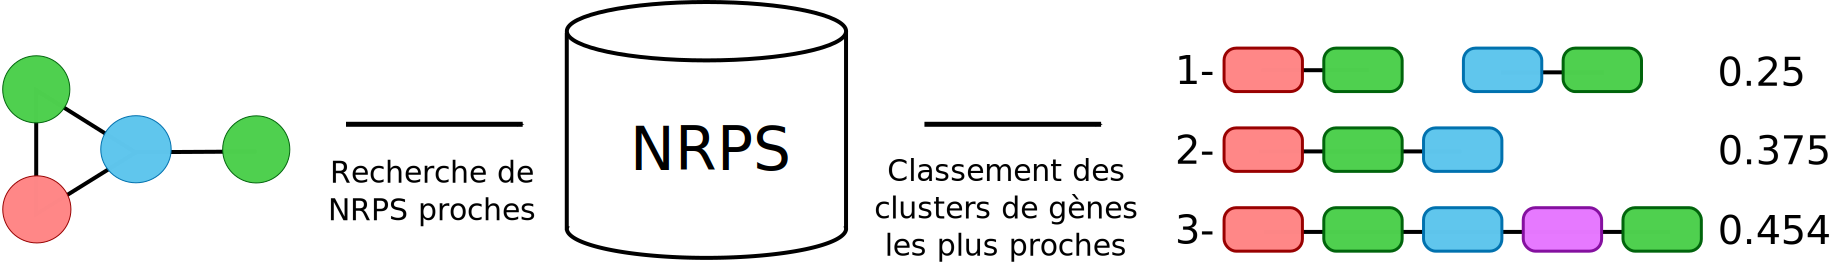
\includegraphics[width=450px]{Figures/synthese/recommandation.png}
    \caption{\label{reco}Processus de recommandation de clusters de gènes proches pour la création d'un NRP souhaité.
    Le logiciel prend en entrée un NRP que l'on souhaite synthétiser.
    Il doit chercher au sein d'une base de NRPS existantes, celles qui produisent le NRP le plus proche du NRP souhaité et classer les meilleurs résultats dans l'ordre de ressemblance.
    Ces clusters proches devraient pouvoir aider les biologistes à choisir des NRPS suffisamment proches du NRP souhaité pour pouvoir les dériver le plus facilement possible.}
  \end{center}
\end{figure}

Le logiciel devra prendre un NRP en entrée et fournir une liste de clusters de gènes en sortie, c'est à dire effectuer une recommandation (voir figure \ref{reco}).
Pour commencer simplement, nous étudierons uniquement la présence ou absence de domaines A dans la NRPS.
À partir des différents domaines NRPS existants et des monomères présents dans le NRP d'intérêt nous établirons une distance.
Cette distance permettra d'ordonner les clusters les uns par rapport aux autres.
Prenons l'exemple d'un peptide d'intérêt contenant de nombreux monomères dont une unique leucine.
Prenons également deux clusters de gènes identiques à l'exception d'un domaine A.
Dans le premier cluster, ce domaine A inclus une leucine alors que le second non et aucun des autres domaines A ne recrute ce monomère.
Alors, la distance que nous allons établir devra donner un meilleur score de proximité au premier cluster.

\subsubsection{Recherche par fingerprint}

L'approche que nous avons utilisé est une approche par fingerprint.
En informatique, les fingerprints sont des structures représentant des données complexes par une projection de ces données à certaines de leurs caractéristiques essentielles.
Dans notre cas, un fingerprint est un vecteur représentant la composition d'un NRP ou d'une NRPS.
Dans le cas des NRP c'est la composition en monomères qui nous intéresse et dans le cas des NRPS la composition en domaines A.
La composition peut être, par exemple, un simple comptage de chacun des monomères, un comptage de tous les dimères, de tous les trimères etc.

\begin{figure}[h!]
  \begin{center}
    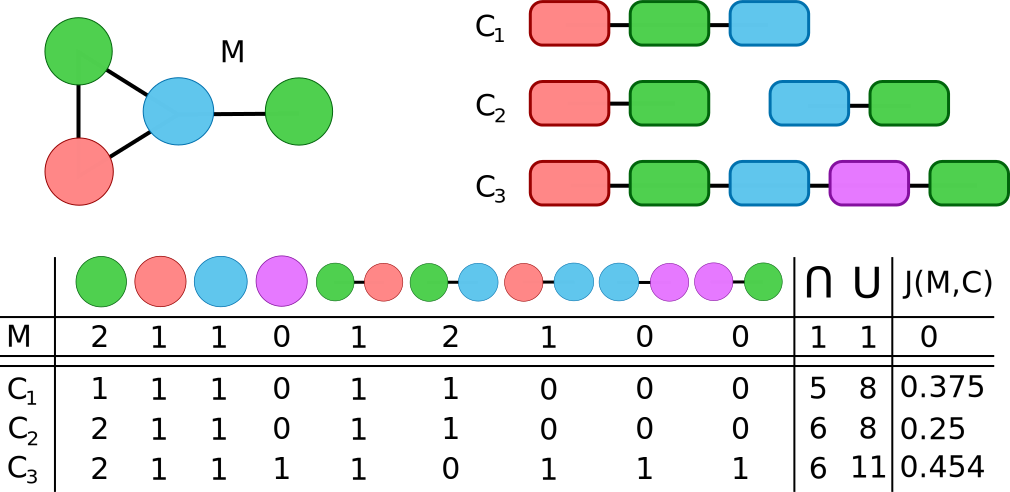
\includegraphics[width=450px]{Figures/synthese/fingerprints.png}
    \caption{\label{jaccard}Exemple de calcul de distance entre un peptide P et trois clusters de gènes $C_1$, $C_2$ et $C_3$.
    Les clusters de gènes sont représentés par une suite de modules colorés en fonction de la couleur du monomère qui sera inclus.
    Dans le tableau sont présents les différents fingerprints pour le monomère et les clusters accompagnés du calcul de la distance de Jaccard.}
  \end{center}
\end{figure}

Dans notre cas, le vecteur sera composé des comptages de monomères seuls et des comptages de dimères (voir schéma \ref{jaccard}).
Pour le NRP, il est très simple d'obtenir ce vecteur.
Chaque monomère est compté indépendamment puis chaque lien est compté comme un dimère comportant les deux monomères liés.
Un dimère A-B est équivalent à un dimère B-A.
Pour les NRPS, nous ne connaissons pas tous les voisinages.
La connaissance actuelle du fonctionnement des enzymes NRPS ne nous permet pas tout le temps de prédire les emplacements exacts de cyclisation.
Les règles générales d'assemblage de différents sous peptides créés par différents gènes NRPS, ne sont pas facilement identifiables.
La première partie des comptages est facile à obtenir.
En analysant les domaines A, il est possible de déterminer leur spécificité (via par exemple NRPSPredictor) et ainsi d'augmenter la valeur de la case correspondant au monomère dans le vecteur.
Pour ce qui est des dimères, il faut analyser les gènes NRPS.
Deux domaines A dans deux gènes différents ne doivent pas générer de dimères.
Nous ajoutons uniquement des dimères pour deux modules A successifs trouvés dans un même gène.

% Etude comparative de la distribution florale dans une portion des Alpes et du Jura

Une fois les vecteurs formés, il faut pouvoir comparer le fingerprint NRP aux fingerprints des clusters.
Pour cela, nous avons choisi de comparer les fingerprints NRPS un à un avec le NRP et de calculer les distances les séparant.
Cette distance permettra de classer les clusters par proximité et de ainsi proposer les plus proches du NRP.
Pour générer cette distance il est nécessaire de prendre en compte à la fois les présences communes entre deux fingerprints mais également les divergences.
Pour répondre à ce besoin, nous avons choisi d'utiliser une distance de Jaccard~\cite{jaccard_etude_1901}.
La distance de Jaccard compare la présence de critères communs entre les deux vecteurs par rapport au nombre de critères totaux.
Dans notre cas nous comparerons les monomères et dimères communs à ceux divergents.

\begin{equation}
  J(A,B) = 1 - \frac{A \cap B}{A \cup B}
\end{equation}

Sur la figure \ref{jaccard}, on peut voir l'application de cette formule à trois clusters de gènes.
Prenons l'exemple du cluster $C_1$.
Ce cluster est composé de 3 domaines A chaînés : un rouge puis un vert et enfin un bleu.
Le vecteur fingerprint représentant ce cluster est composé de 5 valeurs non nulles.
Ces valeurs correspondent aux comptages de chacun des domaines A et des différents dimères de ces domaines.
Ce vecteur diverge de celui correspondant au peptide par 1 vert et deux dimères manquants.
Au total, son indice de Jaccard vaut $5 / 8$, ce qui donne une distance de Jaccard de $1 - 5/8 = 0.375$.





\subsubsection{Tester le modèle}

Afin de tester le modèle nous avons choisi de prendre des peptides réels présents dans Norine.
À partir de ces peptides, nous espérons retrouver leur vrai cluster de gènes au sein d'un ensemble de clusters.
Pour cela, il nous est nécessaire de constituer une base de données test.
Malheureusement, la constitution d'une telle base est très difficile.
Il existe en effet très peu de sources de données mettant en relation des NRP constatés dans l'environnement avec des NRPS réelles.
Nous devons constituer cette base par nous même.

La première piste que nous avions envisagée était de rassembler des données NRPS sûres (annotées manuellement) pour ne pas nous préoccuper de la qualité des données.
Nous avons donc utilisé les données des couples gènes/NRP de MiBIG.
L'intérêt des données issues de MIBiG sont qu'elles ont été entrées manuellement, c'est à dire que le contributeur avait suffisamment confiance en ses données pour les partager avec la communauté.
Cependant, il possible que le contributeur ait entré directement les résultats d'une prédiction sans ajouter d'annotations car celles-ci suffisaient pour ses travaux.
Il nous faut donc vérifier la pertinence des structures NRP présentes en base.
Pour cela nous avons effectué une validation croisée des peptides avec Norine.
Malheureusement, sur les quelques centaines de couples NPRS/NRP décrits dans MIBiG, seuls 60 NRP sont également présents dans Norine.
Pour augmenter leur nombre, il sera nécessaire de valider d'autres structures manuellement.
De plus, les données qui ont été soumises sont structurées différemment selon les contributeurs.
MIBiG laisse une grande liberté dans les champs possibles à l'annotation, ce qui fait que plusieurs utilisateurs entrent des informations semblables sous différents noms.
Cette diversité de structuration dans les fichiers d'annotation empêche la gestion automatique d'un grand nombre d'entrées.
Suite au retrait des annotations impossibles à traiter dans un script (à moins de leur consacrer une exception), environ la moitié des liens potentiels entre Norine et MiBIG ne sont plus présentes.
Ces deux contraintes cumulées nous ont poussé a changer de stratégie et ainsi changer notre jeu de données pour des données issues de prédictions.

% Cette source de données a été un double échec.
% Premièrement, les données téléchargées ne sont pas normalisées.
% Par exemple, les noms des monomères assemblés par une NRPS sont parfois complets et parfois résumés à quelques lettres.
% Ces mêmes monomères peuvent également être présents sous plusieurs noms sans avoir aucun lien entre eux.
% Enfin, les données json ne sont pas non plus toutes structurées de la même manière.
% De ce fait, de nombreuses données ont dues être écartées car portant trop de contraintes pour des exploitations automatiques.
% Le second problème majeur est que quasiment aucun des clusters de gènes restant n'a le NRP correspondant sur Norine.
% Les structures ne peuvent donc pas être contrôlées et confirmées.
% C'est à la suite de tout ces problèmes que nous avons choisi de changer de source de données pour nous tourner vers des annotations éventuellement moins fiables.

A l'aide de Kai Blin (chercheur de l'équipe de Tilmann Weber), nous avons utilisé antiSMASH pour générer des annotations de NRPS sur l'ensemble des génomes de bactéries présentes sur le NCBI.
Ce second jeu de données est beaucoup plus abondant que le premier mais pose également un problème de qualité.
Il n'existe par exemple aucun lien entre les NRP de Norine et les génomes qui ont été analysés.
Il faut faire manuellement les rapprochements pour connaitre les binômes NRP/NRPS.
De plus, les annotations de antiSMASH sont des prédictions et n'ont donc été vérifiées par personne.
Par exemple, de nombreux petits clusters de gènes ne contiennent qu'un ou deux domaines A et il est difficile voire impossible de savoir s'ils sont artefactuels ou mal annotés.

Le programme a été lancé sur les jeux de donnés précédemment présentés dans cette section.
Les problèmes évoqués pour ces jeux de données ne nous permettent pas pour le moment de dégager une quelconque conclusion sur la qualité de prédiction du modèle.
Il est très difficile de donner les causes précises de ces résultats mais ils sont sans doute un cumul de beaucoup de facteurs.
Premièrement, le fait de ne pas connaître les ``vrais'' clusters par avance ne nous permet pas de faire la différence entre un cluster non retrouvé et un cluster inexistant dans les données d'origine car non annotés.
Deuxièmement, les clusters annotés que nous utilisons sont très bruités à cause des prédictions.
Ce bruit nuit forcément à la qualité des fingerprints et augmente les distances artificiellement.
Troisièmement, le modèle que nous avons développé ne prend en compte que les domaines A.
Nous savons qu'une partie de l'information est portée par les autres domaines et c'est un critère qu'il nous faudra intégrer pour mieux rendre compte de la réalité.
Enfin, la distance de Jaccard n'est pas forcément très adaptée au problème et il nous faudra tenter des alternatives issues des systèmes de recommandation classiques.


\subsubsection{Perspectives}

Ce travail est un travail en cours et les résultats présentés ici sont encore très préliminaires.
Malgré les critiques que nous venons de porter au modèle et aux données, il est très encourageant de retrouver quelques résultats positifs lors de ces premiers tests.
Par exemple, s2m permet de connaître le type de liaison entre deux monomères, ce qui n'est pas forcément le cas depuis une annotation manuelle à disposition en ligne.
Cette connaissance pourrait être exploitée afin de rechercher les parties de NRPS effectuant ces liaisons.
Pour pouvoir continuer ce travail, il nous sera également nécessaire de constituer une base d'apprentissage de référence bien annotée.
En effet, sans ces tests nous ne pourrons jamais déterminer avec précision la qualité des algorithmes développés.
Nous sommes actuellement en train de réfléchir à des moyens de constituer ce jeu de données qui pourrait être d'une grande valeur pour de nombreuses tâches.
La solution qui commence à émerger s'appuie sur plusieurs bases de données existantes.
En utilisant à la fois Norine pour les NRP, MIBiG pour les annotations NRPS et le NCBI pour les séquences ADN, nous pouvons créer tout un système d'interconnexion donnant rapidement accès à toutes les informations.
De notre côté nous commençons un long travail de recensement de NRPS correspondants aux peptides de Norine.
En soumettant sur MIBiG les annotations NRPS trouvées depuis et en concrétisant le lien depuis les pages des peptides, il nous est possible de démarrer ce jeu de données.